\pagebreak

\section{Mô hình của đề xuất OHGesture}
\label{sec:ohgesture}

\begin{figure}[H]
	\centering
		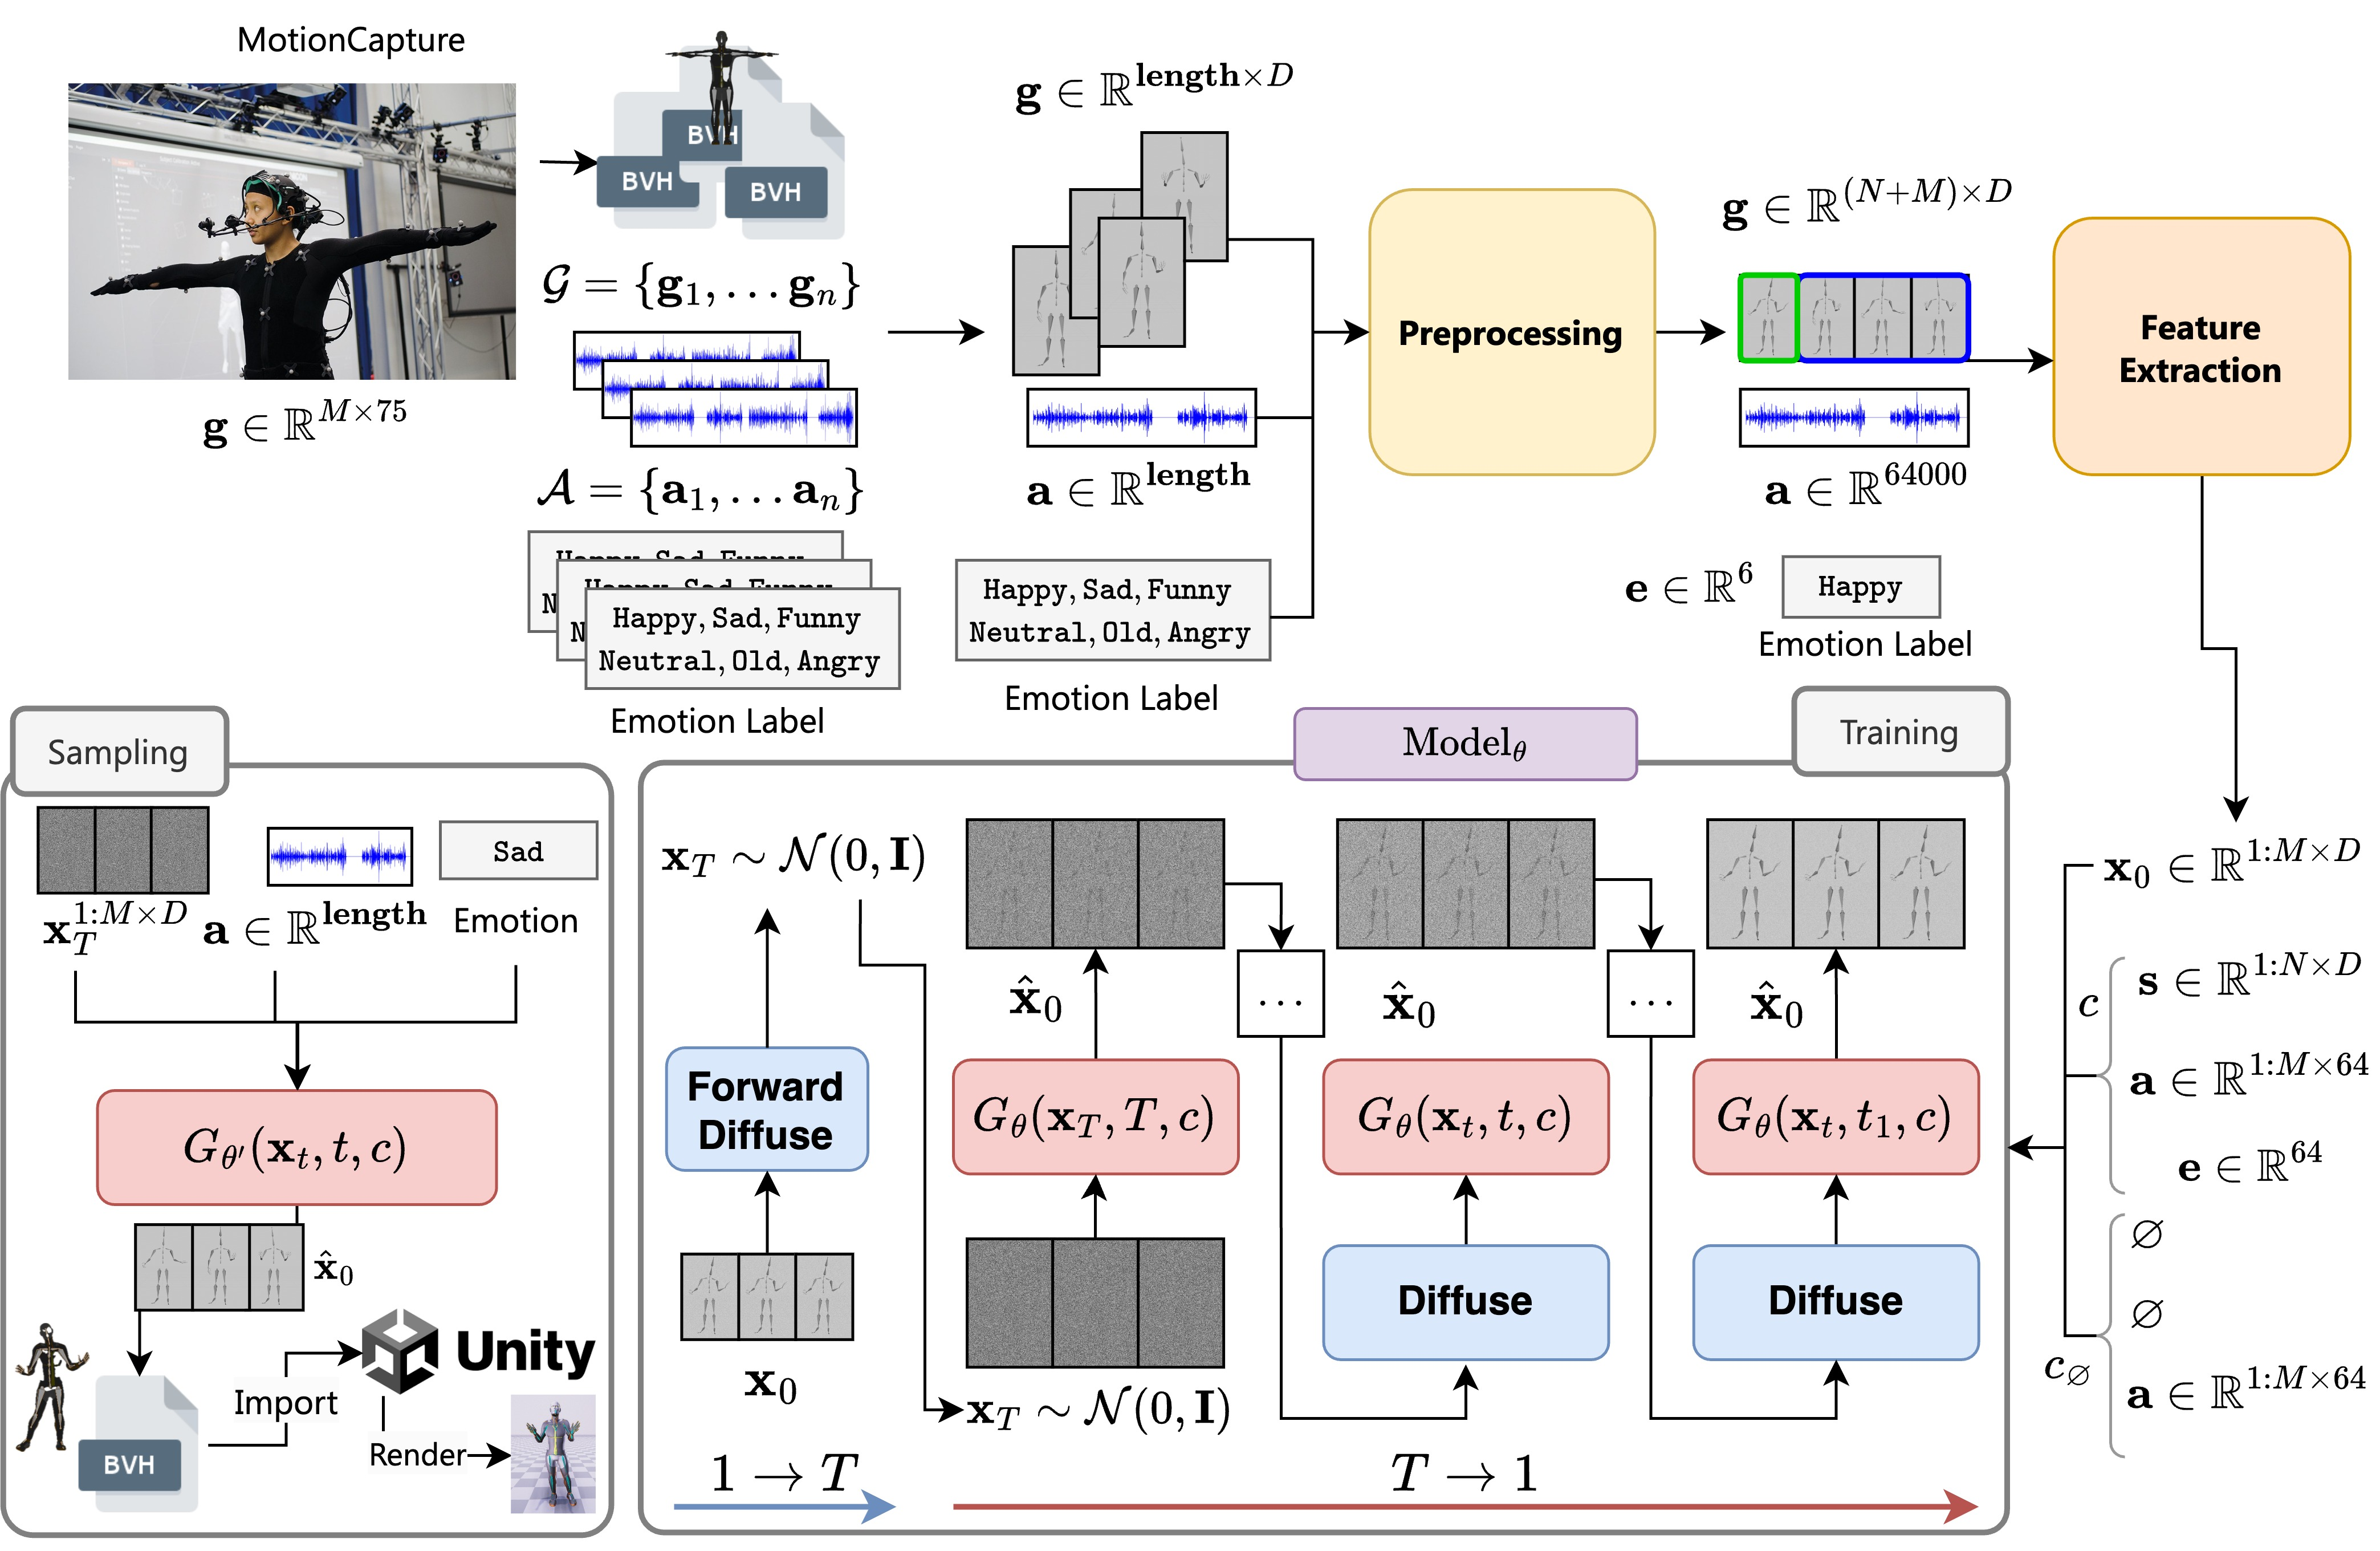
\includegraphics[width=\linewidth]{AllStage}
	\caption{Tổng quan về mô hình OHGesture}
	\label{fig:TrainingAndSampling}
\end{figure}

Mô hình đề xuất \textbf{OHGesture} (\textbf{O}pen \textbf{H}uman \textbf{Gesture} Generation) của luận văn được dựa trên mô hình \textbf{DiffuseStyleGesture} \cite{yang2023diffusestylegesture} áp dụng mô hình Diffusion \cite{ho2020denoising} có điều kiện \cite{ho2022classifier} (Classifier-Free Diffusion Guidance) để điều khiển các đặc trưng trong quá trình khử nhiễu.

Những điểm giống và khác của việc áp dụng mô hình diffusion cho bài toán sinh cử chỉ (gesture generation) so với mô hình Diffusion trong bài toán sinh ảnh:

\vspace{10pt}

\textbf{Điểm giống}
\begin{itemize}
	\item Sử dụng mô hình Diffusion (\autoref{sec:summary_diffusion}) trên cử chỉ $\bx^{1:M \times D}$,  với $M$ frame theo thời gian, $D=1141$ là các điểm tọa độ chuyển động của mỗi khung hình (tương tự width và height trong ảnh).
	\item Sử dụng Diffusion có điều kiện (\autoref{subsec:DiffusionCondition}) với $\bx_0$ objective (\autoref{subsec:X0Objective}).
	\item Ở công đoạn \textit{4. Mã hóa đặc trưng} và công đoạn \textit{6. Giải mã đặc trưng} \autoref{fig:CommonStage}, mô hình sử dụng latent vector có số chiều là $256$.
\end{itemize}

\textbf{Điểm khác}

\begin{itemize}
	\item Sinh cử chỉ có điều kiện:
	\begin{itemize}
		\item Điều kiện cảm xúc: $c = \big[ \mathbf{s}, \mathbf{e}, \mathbf{a}, \mathbf{v} \big]$ và $c_{\varnothing} = \big[ \varnothing, \varnothing, \mathbf{a}, \mathbf{v}\big]$.
		\item Nội suy trạng thái giữa hai cảm xúc $\mathbf{e}_1, \mathbf{e}_2$, sử dụng điều kiện: $c = \big[ \mathbf{s}, \mathbf{e}_1, \mathbf{a}, \mathbf{v} \big]$ và $c_{\varnothing} = \big[ \mathbf{s}, \mathbf{e}_2, \mathbf{a}, \mathbf{v} \big]$.
	\end{itemize}
	\item Ở công đoạn \textit{5. Kết hợp đặc trưng} \autoref{fig:CommonStage}, mô hình sử dụng Self-Attention: Mối liên hệ giữa các cảm xúc, cử chỉ khởi tạo và từng frame (tương tự DALL-E 2 tính mối liên hệ giữa văn bản và ảnh).
	\item Ở công đoạn \textit{5. Kết hợp đặc trưng} \autoref{fig:CommonStage}, mô hình concat giọng nói và văn bản (Tương tự như ControlNet sử dụng Pixel-wise Condition)
	%			\item Học mối liên hệ giữa điều kiện và các frame bằng Local-Cross Attention
\end{itemize}

Trong đó $\bx_0$ là chuỗi $M$ khung hình cử chỉ $\mathbf{x} \in \mathbb{R}^{1:M \times D}$ ($D = 1141$), với điều kiện $c = [\mathbf{s}, \mathbf{e}, \mathbf{a}, \mathbf{v}]$ bao gồm cử chỉ khởi tạo (seed gesture) $\mathbf{s}$,  cảm xúc (emotion) $\mathbf{e}$, chuỗi giọng nói (audio) $\mathbf{a}$ tương ứng cử chỉ, và văn bản  $\mathbf{v}$.

Mục tiêu của mô hình là học được tham số $\theta$ của hàm $G_{\theta}$ (\textbf{g}enerative) với đầu vào là ma trận cử chỉ $\bx^{1:M \times D}_t$, bước thời gian $t$ và điều kiện $c$.
Tổng quan của mô hình đề xuất \textbf{OHGesture} được minh họa ở hình \autoref{fig:TrainingAndSampling}. Tương tự mô hình diffusion cơ bản bao gồm hai quá trình: quá trình tạo nhiễu (diffusion) $q$ và quá trình khử nhiễu (denoising process) $p_{\theta}$ với trọng số $\theta$. Công đoạn \textit{1. Tiền xử lý} sẽ được trình bày ở \autoref{sec:Preprocessing}.

\subsection{Công đoạn xử lý đặc trưng}
Trong công đoạn \textit{2. Xử lý đặc trưng} (\autoref{fig:CommonStage}), mục tiêu là chuyển dữ liệu  thành các ma trận hoặc vector trước khi đưa vào mô hình.

\begin{itemize}
	\item \textbf{Văn bản} (Text):
		Như đã trình bày trong \autoref{subsec:TypicalMethod}, \textit{MDM} \cite{tevet2022human}, \textit{DiffuseStyleGesture+} \cite{yang2022DiffuseStyleGestureplus} trong công đoạn này sử dụng các đoạn văn bản mô tả cử chỉ như là Prompt của Midjourney làm đầu vào cho mô hình, tuy nhiên văn bản mô tả được dùng để phân cụm từng cử chỉ. Trong khi mục tiêu của luận văn là sử dụng văn bản như là một đặc trưng ngữ nghĩa, để căn chỉnh từng đoạn văn bản tương ứng với  từng đoạn cử chỉ phục vụ cho việc xây dựng người kỹ thuật số.
		
		Vì vậy, trong công đoạn này đóng góp của luận văn là sử dụng dữ liệu tiếng nói có sẵn, sau khi tiền xử lý ở \autoref{sec:Preprocessing} để thu được văn bản,  luận văn sử dụng mô hình FastText  \cite{bojanowski2017enriching} để nhúng (embedding) văn bản thành các vector căn chỉnh tương ứng với số frame tương ứng với cử chỉ. Với các vùng không có văn bản sẽ được cho là ma trận $\mathbf{0}$, các vùng có từ vựng tương ứng sẽ được gán là giá trị nhúng  theo từng khung hình của cử chỉ để được ma trận văn bản $\mathbf{v}^{1:M \times 300}$.
		
		\item \textbf{Giọng nói} (Speech): Tất cả dữ liệu giọng nói ở dạng wav sẽ được giảm số sample rate (downsampled) xuống $16 \mathrm{kHz}$, và giọng nói sẽ được lấy tương ứng với cử chỉ là 4s để được vector $\mathbf{a} \in \mathbb{R}^{64000}$. Tương tự DiffuseStyleGesture, luận văn sử dụng mô hình pre-train WavLM Large \cite{Chen_2022} nhúng waveform thô vào để được vector thể hiện đặc trưng âm thanh. Sau đó sử dụng nội suy tuyến tính (interpolation) để căn chỉnh đặc trưng của vector tiềm ẩn trong WavLM theo chiều thời gian thành $20 \text{fps}$ để được ma trận giọng nói $\mathbf{a} \in \mathbb{R}^{1:M \times 1024}$
		
		\item \textbf{Cảm xúc} (Emotion): Cảm xúc là nhãn được chọn 1 trong 6 cảm xúc bao gồm: $\texttt{Happy}$, $\texttt{Sad}$, $\texttt{Neutral}$, $\texttt{Old}$, $\texttt{Relaxed}$ và $\texttt{Angry}$. 
		
		Sau đó nhãn cảm xúc được đi qua lớp one-hot encoding để được vector  $\mathbf{e} \in \mathbb{R}^{6}$.
		
%		bao gồm 6 cảm xúc khác nhau được biểu diễn thành một vector theo phương pháp one-hot encoding, 
		
%		sau đó luận văn đưa qua một vector tuyến tính để được vector đặc trưng $\mathbf{E} \in \mathbb{R}^{64}$. Mục tiêu là để có thể concat được với vector khởi tạo $\mathbf{S} \in \mathbb{R}^{192} $ để tạo thành vector tiềm ẩn $256$ chiều. $\mathbf{E} \in \mathbb{R}^{64}$
		
		\item \textbf{Cử chỉ khởi tạo}: Cử chỉ khởi tạo (seed gesture) $\mathbf{s} \in \mathbb{R}^{1:N \times D}$ có được từ cử chỉ ground truth $
		\mathbf{g} \in \mathbb{R}^{(N+M) \times D}$, với mỗi frame là dữ liệu bao gồm $75$ khớp xương, được xử lý theo công thức \autoref{eq:gesturevector} để được vector $1141$ chiều, trình bày ở công thức \autoref{eq:gesturevector}. Mô hình của luận văn cắt $N = 8$ frame đầu để làm cử chỉ khởi tạo $\mathbf{s} \in \mathbb{R}^{1:N \times D} $
		
		\item \textbf{Cử chỉ thật}: Tương tự cử chỉ khởi tạo, từ $
		\mathbf{g} \in \mathbb{R}^{(N+M) \times D}$, luận văn sử dụng $M = 80$ (4 giây với $20fps$) frame là dữ liệu cử chỉ thật $\mathbf{x}_{0} \in \mathbb{R}^{1:M \times D}$. 
\end{itemize}
%, sau đó sử dụng một lớp tuyến tính để giảm kích thước của đặc trưng xuống còn vector đặc trưng với $64$ để tạo thành ma trận cuối cùng $\mathbf{A} \in \mathbb{R}^{M \times 64}$.

\subsection{Công đoạn trích xuất đặc trưng}
\label{subsec:feature_extraction}

Trong công đoạn \textit{3. Trích xuất đặc trưng} (\autoref{fig:CommonStage}), mục tiêu là chuyển ma trận thành các vector tiềm ẩn (latent vector) biểu diễn thông tin của dữ liệu bằng cách cho các đặc trưng cần học đi qua các lớp biến đổi tuyến tính (linear) hoặc MLP (Multilayer Perceptron).

\begin{figure}[H]
	\centering
	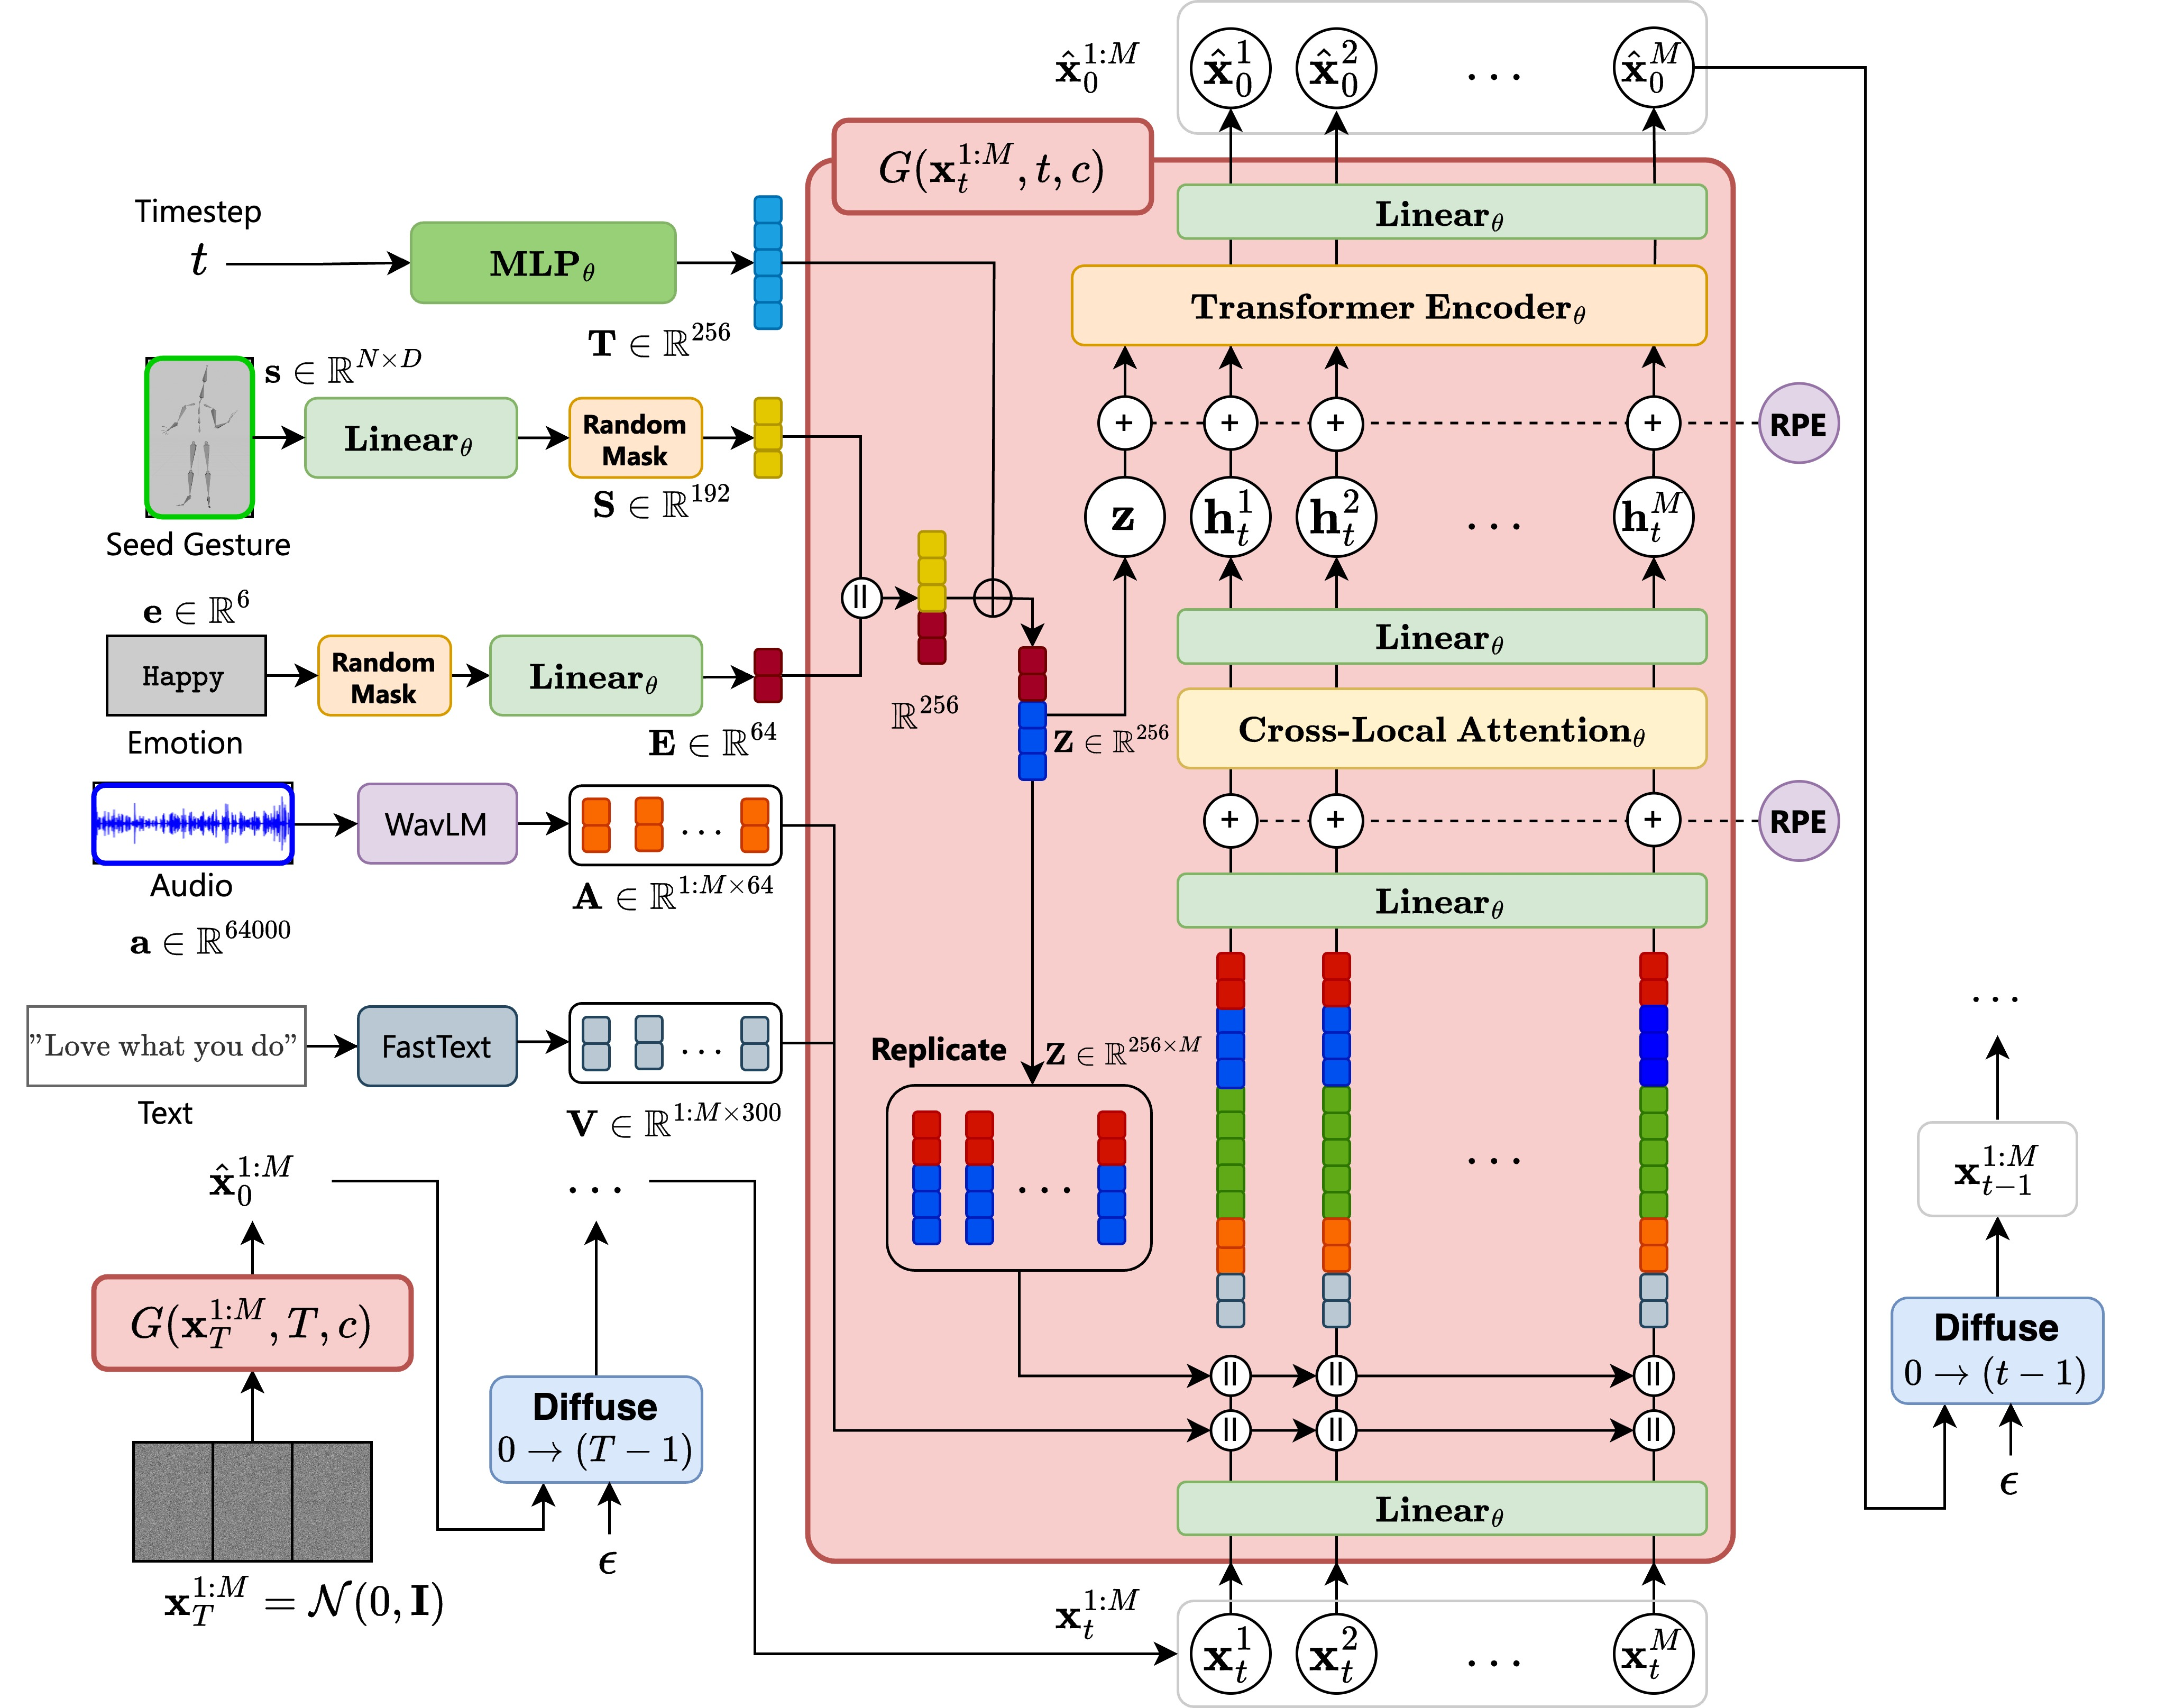
\includegraphics[width=\textwidth]{OHGesture}
	\caption{Mô hình trong OHGesture}
	\label{fig:OHGesture}
\end{figure}
\vspace{-10pt}

\begin{itemize}
	\item \textbf{Bước thời gian $\mathbf{T} \in \mathbb{R}^{256}$ }: Bước thời gian ở mỗi quá trình $t \in [0, T]$, mục tiêu của mô hình là để với bước thời gian $t$ bất kỳ, mô hình có thể tổng quát hóa quá trình khử nhiễu, và có thể học được việc với từng bước $t$ thì giá trị sẽ thay đổi thế nào đối với kết quả dự đoán $\bx_0$. Giá trị timestep $t$ được khởi tạo bằng việc mã hóa nhúng vị trí (Position Embedding) bằng hàm sinusoidal $\text{PE}(t) = \left[ \sin{\left(\frac{t}{10000^{2i / d}}\right)}, \cos{\left(\frac{t}{10000^{2i / d}}\right)} \right]$, sau đó được đưa vào một MLP (Multilayer perceptron) để biến đổi thành vector $\mathbf{T}  \in \mathbb{R}^{256}$.
	
	  \item \textbf{Giọng nói $\mathbf{A} \in \mathbb{R}^{1:M \times 64}$}: Từ giọng nói $\mathbf{a} \in \mathbb{R}^{1:M \times 1024}$ sẽ đi qua một lớp tuyến tính (linear layer) để giảm kích thước của đặc trưng xuống còn vector đặc trưng $64$ để tạo thành ma trận cuối cùng $\mathbf{A} \in \mathbb{R}^{1:M \times 64}$.
	  
	  \item \textbf{Văn bản $\mathbf{V} \in \mathbb{R}^{1:M \times 64}$}: Văn bản $\mathbf{v}^{1:M \times 300}$ sẽ được đi qua lớp tuyến tính (linear layer) để căn chỉnh tương ứng với vector âm thanh.
	
	\item \textbf{Cử chỉ khởi tạo $\mathbf{S} \in \mathbb{R}^{192}$}: Từ $\mathbf{s} \in \mathbb{R}^{1:N \times D}$ sẽ được đi qua một lớp tuyến tính (linear layer) để được vector $\mathbf{S} \in \mathbb{R}^{192}$, vector $\mathbf{S}$ sau đó được đi qua một lớp mặt nạ ngẫu nhiên (random mask) trong quá trình huấn luyện để bỏ trong trường hợp nếu một trong $N$ frame bị thiếu thì sẽ ảnh hưởng như thế nào đến cử chỉ dự đoán.

  \item \textbf{Cảm xúc $\mathbf{E} \in \mathbb{R}^{64}$}: Từ vector cảm xúc $\mathbf{e} \in \mathbb{R}^{6}$ sẽ được đưa qua lớp tuyến tính (linear layer) để được vector đặc trưng $\mathbf{E} \in \mathbb{R}^{64}$. Mục tiêu là để có thể concat được với vector khởi tạo $\mathbf{S} \in \mathbb{R}^{192} $ để tạo thành vector tiềm ẩn $256$ chiều.
  
	\item \textbf{Cử chỉ nhiễu $\mathbf{x}_{T} \in \mathbb{R}^{1:M \times D}$} (Noisy gesture): khi huấn luyện, $\mathbf{x}_{t}$ là cử chỉ nhiễu có cùng kích thước như cử chỉ gốc $\mathbf{x}_{0}$ sẽ được sinh ngẫu nhiên từ phân phối chuẩn $\mathcal{N}(0, \mathbf{I})$. Khi sinh ngẫu nhiên, cử chỉ nhiễu ban đầu $\mathbf{x}_{T}$ được lấy mẫu từ phân phối Gaussian và các $\mathbf{x}_{t}, t<T$ khác là kết quả của bước làm nhiễu trước đó như \autoref{fig:TrainingAndSampling}.
%	Sau đó, kích thước được điều chỉnh thành 256  bằng lớp biến đổi tuyến tính (linear layer).
\end{itemize}


\subsection{Công đoạn mã hóa đặc trưng}

Trong công đoạn \textit{4. Mã hóa đặc trưng} (\autoref{fig:CommonStage}), mục tiêu là giảm số chiều của dữ liệu xuống kích thước thấp hơn, nhằm giảm việc bùng nổ khối lượng tính toán.

Với dữ liệu chính trong quá trình Diffusion chính là chuỗi cử chỉ $\bx_t \in \mathbb{R}^{1:M \times D}$. Như minh họa ở \autoref{fig:OHGesture}, chuỗi cử chỉ với kích thước $M \times D$ sẽ đi qua lớp $\operatorname{Linear}_{\theta}$ để được ma trận $\mathbf{X} \in \mathbb{R}^{1:M \times 256}$. Quá trình giảm chiều dữ liệu của $\bx$ sẽ được thực hiện trước khi chuỗi cử chỉ $\bx$ đi qua các lớp Cross-Local Attention và Transformer Encoder để tính sự tương quan giữa nhiều loại dữ liệu khác nhau.


\subsection{Công đoạn kết hợp đặc trưng}

Trong công đoạn \textit{5. Kết hợp đặc trưng} (\autoref{fig:CommonStage}), mục tiêu là sử dụng các phép concat, cộng hoặc các lớp attention để tính sự tương quan giữa các đặc trưng.

Đầu tiên cử chỉ khởi tạo $\mathbf{S} \in \mathbb{R}^{192}$ và vector cảm xúc $\mathbf{E} \in \mathbb{R}^{64}$ được ghép lại với nhau để tạo thành một vectơ có kích thước $256$, bởi vì kích thước $256$ là kích thước vector tiềm ẩn được chọn để tính tương quan giữa các đặc trưng. Sau đó được cộng thêm vector timestep $\mathbf{T}$ để tạo thành vector $\mathbf{z} \in \mathbb{R}^{256}$.

\begin{equation}
	\label{eq:ConditionConcat}
	\mathbf{z}_{tk} = \operatorname{concat }(\mathbf{E}\ || \  \mathbf{S}) + \mathbf{T}
\end{equation}

\subsubsection{Kết hợp đặc trưng theo khung hình}

Sau đó, $\mathbf{z}$  replicate $M$ lần để căn chỉnh kích thước tương đương với kích thước khung hình để được $\mathbf{Z} \in \mathbb{R}^{1:M \times 256}$

Ta sẽ cộng ma trận giọng nói và văn bản với nhau để được ma trận kết hợp thông tin của văn bản và giọng nói. Sau đó tiếp tục kết hợp concat với ma trận cử chỉ $\mathbf{X}$. Cuối cùng kết hợp với ma trận $\mathbf{Z}$ để được ma trận $\mathbf{H}$.

\begin{equation}
	\label{eq:FrameConcat}
	\mathbf{M} = \operatorname{concat}( \mathbf{Z}\  || \   \operatorname{concat}(\mathbf{X}\ || \  (\mathbf{V} + \mathbf{A}) ) )
\end{equation}

Sau khi có ma trận $\mathbf{M} \in \mathbb{R}^{1:M \times P}$ theo \autoref{eq:FrameConcat} thể hiện đặc trưng theo khung hình từ frame $1$ đến frame $M$, với mỗi frame có kích thước $P$ là tổng của các đặc trưng đã concat. Với $\mathbf{X} \in \mathbb{R}^{1:M \times 256}$, $\mathbf{Z} \in \mathbb{R}^{1:M \times 256}$ và $\mathbf{A}, \mathbf{V} \in \mathbb{R}^{1:M \times 64}$, thì $P$ sẽ có kích thước $256 * 2 + 64$. Sau đó, ma trận $\mathbf{m}$ sẽ được đi qua quá trình biến đổi tuyến tính: $\mathbf{m}^{[1:M] \times 256} = \operatorname{Linear}_{\theta}(M)$ để được ma trận $\mathbf{m} \in \mathbb{R}^{[1:M] \times 256}$.

\subsubsection{Cơ chế attention trong quá trình kết hợp các đặc trưng}

Trong mô hình của luận văn, mục tiêu của việc áp dụng cơ chế attention là tìm được sự tương quan của từng khung hình với nhau.

Lớp attention có công thức như sau:

\begin{equation} \label{eq:attention}
	\operatorname{Attention}(\mathbf{Q}, \mathbf{K}, \mathbf{V}, \mathbf{M})=\operatorname{softmax}\left(\frac{\mathbf{Q} \mathbf{K}^{T}+\mathbf{M}}{\sqrt{C}}\right) \mathbf{V}
\end{equation}

Công thức Attention trên có $\mathbf{Q}$, $\mathbf{K}$ ,$\mathbf{V}$ là các ma trận sau khi đi qua các ma trận biến đối tuyến tính $\mathbf{Q} = \mathbf{X} \mathbf{W}_Q$, $\mathbf{K} = \mathbf{X} \mathbf{W}_K$, $\mathbf{V} = \mathbf{X} \mathbf{W}_V$. Với đầu vào là ma trận biểu thị chuỗi $M$ khung hình, với mỗi khung hình là một vector được concat từ các vector đặc trưng bao gồm cả cử chỉ khởi tạo, văn bản, giọng nói, cảm xúc và cử chỉ $\bx_t$ mà luận văn muốn thực hiện khử nhiễu. Quá trình Local-Cross Attention được điều khiển chỉ để tính các đặc trưng cục bộ của chuyển động của các cử chỉ và đặc trưng trong các khung hình lân cận.

\begin{figure}[H]
	\centering
	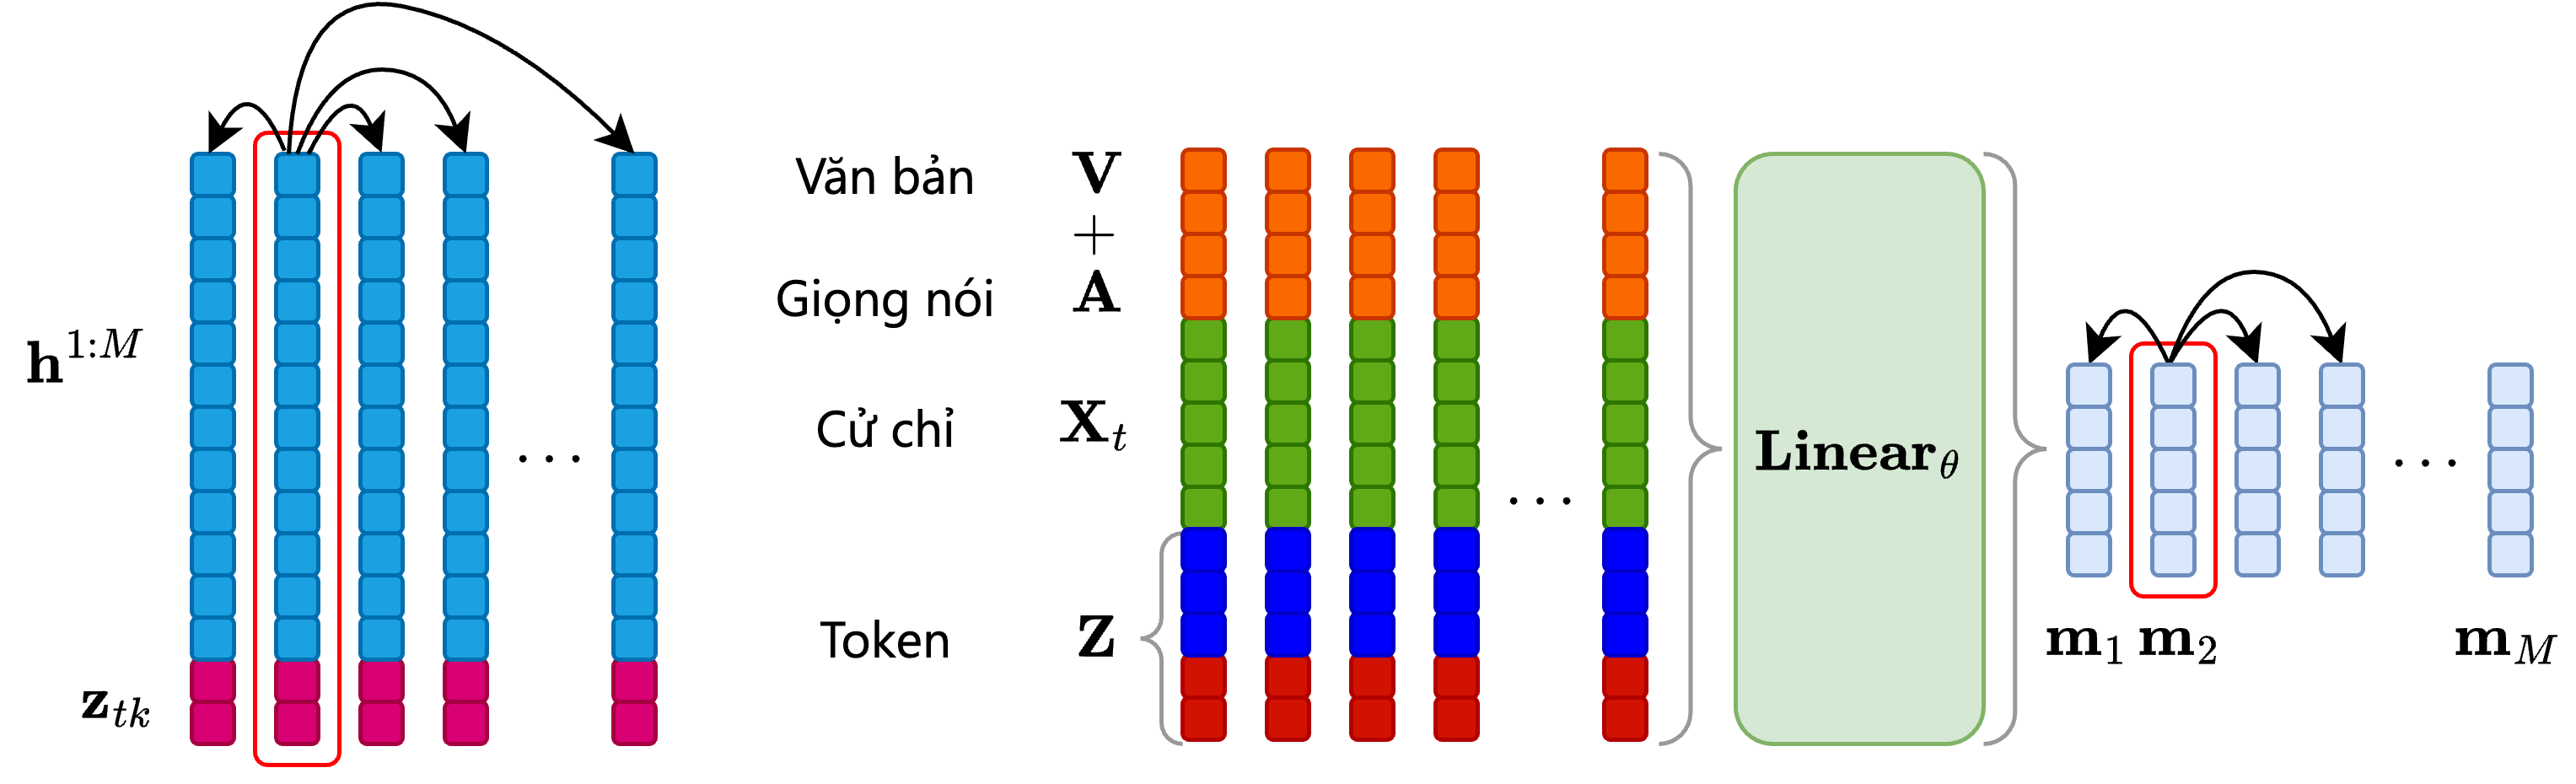
\includegraphics[width=\textwidth]{CrossLocalAttention}
	\caption{Cơ chế Attention trong Transformer Encoder và Cross-Local Attention}
	\label{fig:CrossLocalAttention}
\end{figure}

Hàm Attention hoạt động như một bộ từ điển, với các thông tin cuối cùng tra được là ma trận $\mathbf{V}$ (value), còn $\mathbf{Q}$ (query) là từ khóa muốn tìm kiếm, $\mathbf{K}$ (key) là danh mục các từ khóa trong bộ từ điển tra cứu. Quá trình Attention sẽ tính toán mức độ tương đồng giữa \( \mathbf{Q} \) và \( \mathbf{K} \) để xác định trọng số cho các giá trị trong \( \mathbf{V} \). 

Kết quả cuối cùng là tổ hợp các giá trị trong \( \mathbf{V} \), trong đó các giá trị tương ứng với các khóa giống truy vấn nhất sẽ có trọng số cao hơn. $\mathbf{M}$ là mặt nạ (mask) để thực hiện quá trình chú ý cục bộ. Cross-Local Attention sẽ được minh họa như \autoref{fig:CrossLocalAttention} bên phải. Còn lớp Transformer Encoder sẽ sử dụng Self-Attention lớp bên trái.

\subsubsection{Kết hợp đặc trưng cục bộ với Cross-Local Attention}

Ma trận $\mathbf{m} \in \mathbb{R}^{[1:M] \times 256}$ sẽ tiếp tục đi qua lớp Cross-Local Attention để tính tương quan giữa các đặc trưng cục bộ: 

\begin{equation}
	\mathbf{h}^{1:M}_{t}  = \operatorname{Linear}_{\theta}  ( \operatorname{Cross-Local\ Attention}( \mathbf{m}) )
	\label{eq:CrossLocalAttention}
\end{equation}

Cross-local Attention sẽ thực hiện với $\operatorname{Query} = \operatorname{Key} = \operatorname{Value} = \mathbf{m}$. 
Tương tự ý tưởng từ phương pháp Routing Transformer \cite{roy2021efficient}, Cross-local Attention cho thấy rằng sự quan trọng trong việc xây dựng biểu diễn các vector đặc trưng trung gian trước khi đi qua lớp Transformer Encoder như \autoref{fig:OHGesture}. 
Các vector đặc trưng sẽ được cộng thêm một vector sinusoids hay mã hóa vị trí tương đối (Relative position encoding \cite{vaswani2017attention}) để thể hiện được đặc trưng thời gian trước khi đi qua lớp Cross-Local Attention.


Sau quá trình Cross-Local Attention, mô hình tiếp tục được đưa qua lớp tuyến tính theo \autoref{eq:CrossLocalAttention} để căn chỉnh tương ứng với $M$ khung hình, bao gồm $\mathbf{h}^{1:M}$.


\subsubsection{Kết hợp đặc trưng toàn cục với Transformer Encoder}

\begin{figure}[H]
	\centering
	\begin{subfigure}{0.42\textwidth}
		\centering
		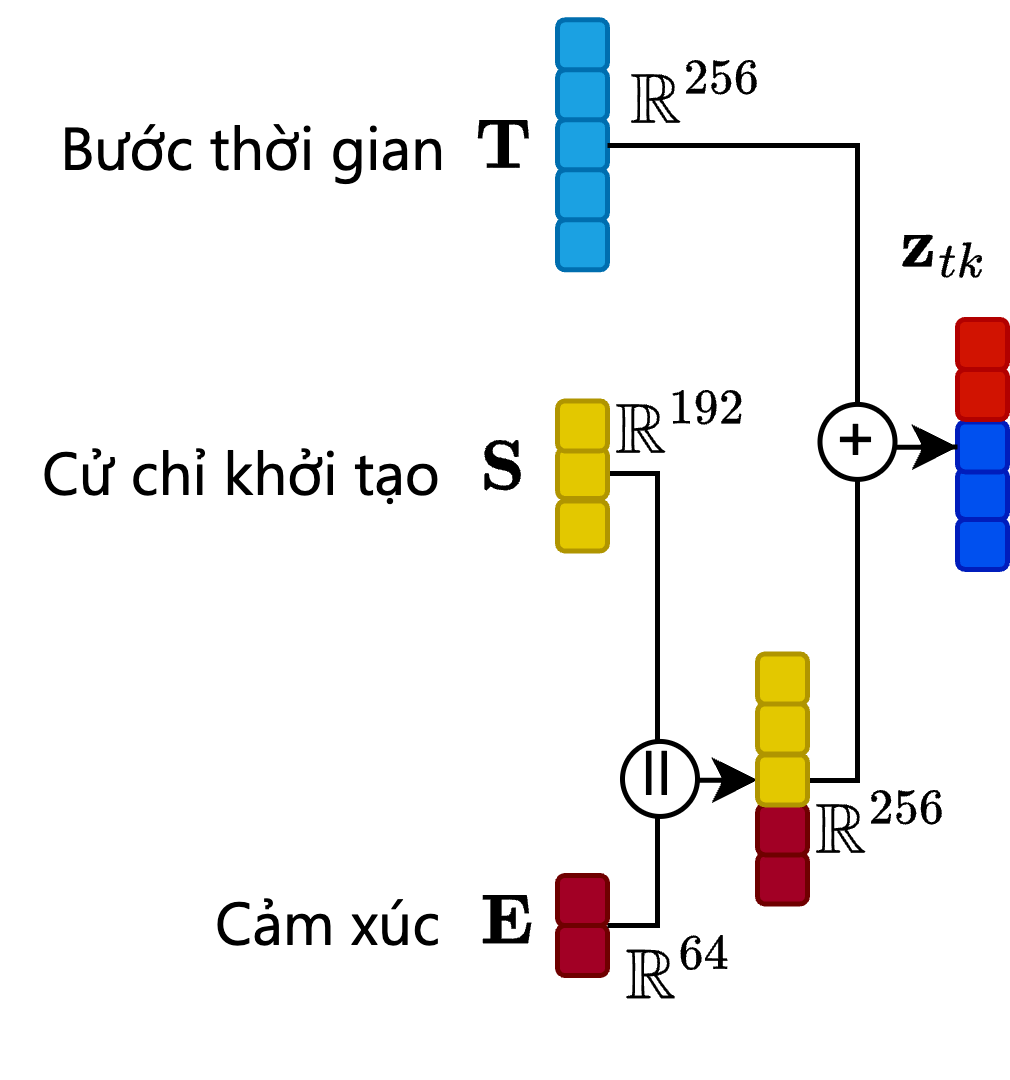
\includegraphics[width=\textwidth]{z}
		\caption{Cách concat đặc trưng để được $\mathbf{z}_{tk}$}
		\label{fig:FeatureFusion}
	\end{subfigure}
	\hfill
	\begin{subfigure}{0.55\textwidth}
		\centering
		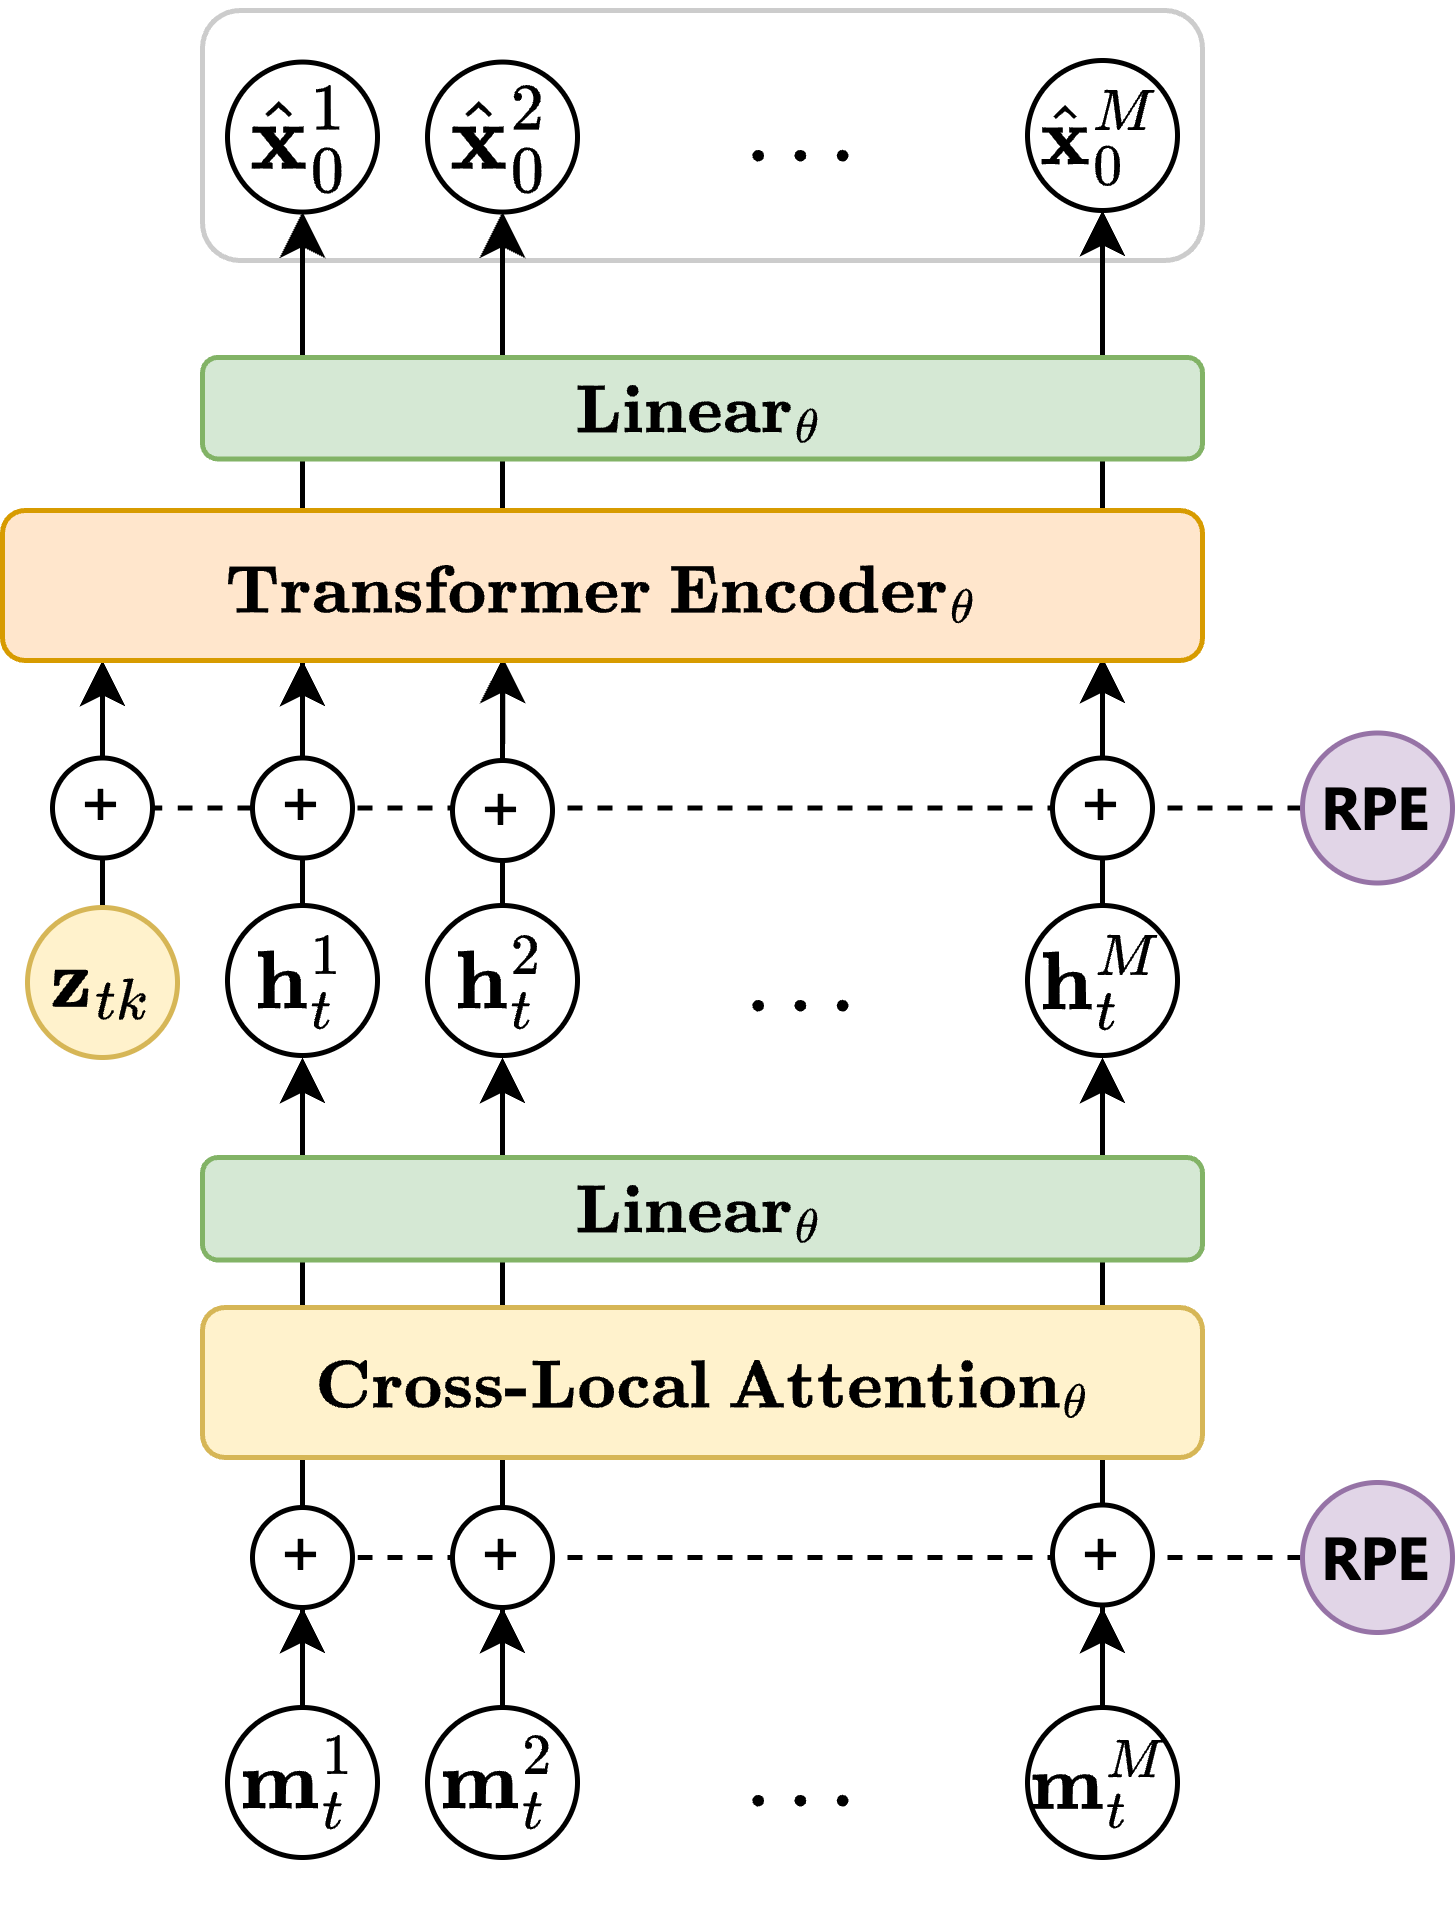
\includegraphics[width=\textwidth]{FeatureFusion}
		\caption{Quá trình kết hợp đặc trưng theo từng frame}
		\label{fig:ZToken}
	\end{subfigure}
\end{figure}


%Sau đó quá trình tương tự như xử lý các vector đặc trưng của mô hình BERT 

Kế thừa từ MDM \cite{tevet2022human}, vector $\mathbf{z}$ là token đầu tiên thể hiện thông tin cho toàn bộ chuỗi khung hình, tương tự như  $z_{\text{tk}}$ trong mô hình BERT \cite{devlin2019bertpretrainingdeepbidirectional}, với token $\texttt{CLS}$ đầu tiên thể hiện thông tin của toàn bộ đoạn văn bản.
Ở đây, luận văn sử dụng $z_{\text{tk}}$ là $\mathbf{z} \in \mathbb{R}^{256}$ (\autoref{eq:ConditionConcat}) token đầu tiên biểu thị đặc trưng biểu thị cho toàn bộ chuỗi $M$ frame.

\begin{equation}
	\mathbf{x}^{1:M}_{0}  = \operatorname{Transformer\ Encoder}( \operatorname{concat}( \mathbf{z}_{tk} \ ||\  \mathbf{h}^{1:M}_{t}  )))
	\label{eq:TransformerEncoder}
\end{equation}


Các vector $\mathbf{h}$ biểu thị cho chuỗi $M$ khung hình, tương tự như phương pháp Reformer \cite{kitaev2020reformer}, trước khi đi vào lớp Self-Attention trong Transformer Encoder, mô hình sẽ sử dụng lớp mã hóa vị trí tương đối (Relative Position Encoding - RPE) để thay thế mã hóa vị trí tuyệt đối, giúp mô hình hiệu quả hơn trong việc xử lý chuỗi dài.
Khi vào lớp Transformer Encoder \cite{vaswani2017attention} giúp tính toán được mối liên hệ giữa các chuỗi dữ liệu. 
Trong lớp Transformer Encoder mô hình sẽ áp dụng cơ chế tự chú ý tương tự như \autoref{eq:attention} trên nhưng không sử dụng mặt nạ. 


\subsection{Công đoạn giải mã đặc trưng}

Trong công đoạn \textit{6. Giải mã đặc trưng} (\autoref{fig:CommonStage}), sau khi tính được sự tương quan giữa các đặc trưng, mục tiêu là tăng kích thước dữ liệu trở về kích thước ban đầu.

Như minh họa ở \autoref{fig:OHGesture}, ma trận tiềm ẩn, sau khi đi qua lớp Transformer Encoder để tính sự tương quan giữa nhiều loại dữ liệu khác nhau. Kết quả sẽ đi qua lớp $\operatorname{Linear}_{\theta}$ để tăng kích thước ma trận tiềm ẩn thành kích thước ban  đầu $\hat{\mathbf{x}}_{0} \in \mathbb{R}^{1:M \times D}$.

Công đoạn cuối cùng, kết xuất sẽ được trình bày ở \autoref{sec:Render}.

\subsection{Điều khiển cảm xúc trong bài toán sinh cử chỉ}

Ở các bước trên mô hình đã có thể học được cách sinh cử chỉ, nhưng để mô hình có thể học được các cảm xúc ở các tình huống khác nhau sẽ được giải quyết bằng cách tham số hóa và lần lượt thay đổi từng cảm xúc để sao cho khi thay đổi cảm xúc thì kết quả dự đoán phải có cảm xúc tương ứng.

Tương tự như các phương pháp sử dụng mô hình khử nhiễu có điều kiện \cite{ho2022classifier}, \cite{tevet2022human}, luận văn sử dụng điều kiện $c = [ \mathbf{s}, \mathbf{e}, \mathbf{a}, \mathbf{v} ]$,  bao gồm cử chỉ khởi tạo $\mathbf{s}$, cảm xúc $\mathbf{e}$, giọng nói tương ứng $\mathbf{a}$ và văn bản $\mathbf{v}$. Mô hình diffusion có điều kiện $c$ ở đây sẽ là tổng cả trường hợp ở từng bước $t$ trong mô hình khử nhiễu $\text{G}_\theta \left( \bx_{t}, t, c \right)$, với  $c_{\varnothing}=[\varnothing, \varnothing, \mathbf{a}, \mathbf{v}]$ không điều kiện và $c = [\mathbf{s}, \mathbf{e}, \mathbf{a}, \mathbf{v}]$ có điều kiện. Quá trình này có thể dễ dàng điều khiển bằng một lớp mặt nạ ngẫu nhiên (random mask) trên các vector đặc trưng của cử chỉ khởi tạo $\mathbf{s}$ và cảm xúc $\mathbf{e}$. Khi đó, mô hình chỉ việc thay đổi nhãn tương ứng với lớp mask đã lấy ngẫu nhiên để mô hình có thể tối ưu theo các điều kiện khác nhau. 


\begin{equation} \label{eq:denoise}
\hat{\bx}_{0 c, c_{\varnothing}, \gamma}=\gamma \cdot G \left(\bx_{t}, t, c\right)+(1-\gamma) \cdot G \left(\bx_{t}, t, c_{\varnothing}\right)
\end{equation}

Điểm đặc biệt là có thể dựa trên việc học có điều kiện và không có điều kiện của classifier-free guidance \cite{ho2022classifier}, có thể nội suy giữa hai cảm xúc $\mathbf{e}_1$ và cảm xúc $\mathbf{e}_2$ khác nhau bằng cách cho điều kiện $c = \left[\mathbf{s}, \mathbf{e}_{1}, \mathbf{a}, \mathbf{v} \right]$ và $c_\varnothing = \left[\mathbf{s}, \mathbf{e}_{2}, \mathbf{a}, \mathbf{v} \right]$. Khi đó ta có thể viết lại $\hat{x}_{0 \gamma, c_{1}, c_{2}}=\gamma  \cdot G \left(x_{t}, t, c_{1} \right)+(1-\gamma) \cdot G \left(x_{t}, t, c_{2}\right)$.


\subsection{Quá trình huấn luyện}


\begin{algorithm}[H]
	\caption{Huấn luyện trong OHGesture}
	\label{alg:trainingohgesture}
	\setlength{\baselineskip}{10pt}
	\begin{enumerate}
		\item Tính sẵn các giá trị và siêu tham số: $\gamma$, $\sqrt{\alpha_t}$, $\sqrt{1 - \alpha_t}$, $\sqrt{\bar{\alpha}_t}$ và nhiễu ngẫu nhiên $\boldsymbol{\epsilon}_t$ tại mỗi bước $t: 1 \rightarrow T$. Định nghĩa lịch nhiễu $\{\alpha_t \in (0, 1)\}_{t=1}^T$.
		
		\item Lấy nhãn ban đầu $\mathbf{x}_0$ từ phân phối dữ liệu đã chuẩn hóa.
		
		\item Tạo ngẫu nhiên các mặt nạ Bernoulli $c_{1} = \big[ \mathbf{s}, \mathbf{e_1}, \mathbf{a}, \mathbf{v} \big]$, $c_{2} = \big[ \mathbf{s}, \mathbf{e_2}, \mathbf{a}, \mathbf{v} \big]$, hoặc $c_{2} = \big[ \varnothing, \varnothing, \mathbf{a}, \mathbf{v} \big]$.
		
		\item Thêm nhiễu để có cử chỉ nhiễu $\mathbf{x}_t$:
		\[
		\mathbf{x}_t = \sqrt{\bar{\alpha}_t} \mathbf{x}_0 + \sqrt{1 - \bar{\alpha}_t} \boldsymbol{\epsilon}_t
		\]
		
		\item Với mỗi bước $t$, lấy \textbf{ngẫu nhiên} $t$ từ $[1, T]$.
		
		\item Với $\mathbf{x}_t$, $t$ và các điều kiện mặt nạ $c_1$, $c_2$, dự đoán chuỗi cử chỉ:
		\[
		\hat{\mathbf{x}}_{0 \gamma, c_{1}, c_{2}} = \gamma \cdot G_{\theta} \left(\mathbf{x}_{t}, t, c_{1}\right) + (1 - \gamma) \cdot G_{\theta} \left(\mathbf{x}_{t}, t, c_{2}\right)
		\]
		
		\item Tính loss và đạo hàm để cập nhật trọng số $\theta$:
		\[
		\mathcal{L}_t = \mathbb{E}_{t \sim [1, T], \mathbf{x}_0, \boldsymbol{\epsilon}_t} \left[ \operatorname{HuberLoss}(\mathbf{x}_0, \hat{\mathbf{x}}_0 ) \right]
		\]
		
		\item Lặp lại từ bước 6 cho đến khi hội tụ, thu được các tham số tối ưu $\theta'$.
	\end{enumerate}
\end{algorithm}


\autoref{alg:trainingohgesture} huấn luyện mô hình OHGesture bắt đầu bằng việc tính toán các giá trị và siêu tham số cần thiết như $\gamma$, $\sqrt{\alpha_t}$, $\sqrt{1 - \alpha_t}$, $\sqrt{\bar{\alpha}_t}$ và nhiễu ngẫu nhiên $\boldsymbol{\epsilon}_t$ cho từng bước thời gian $t$ từ 1 đến $T$. Sau đó, nhãn ban đầu $\mathbf{x}_0$, đại diện cho cử chỉ gốc, được lấy từ phân phối dữ liệu đã chuẩn hóa. Tiếp theo, các mặt nạ Bernoulli $c_1$ và $c_2$ được tạo ngẫu nhiên, mô phỏng các điều kiện khác nhau như cử chỉ, cảm xúc, giọng nói, hoặc văn bản, với một trong các mặt nạ có thể là không có thông tin cảm xúc. Sau khi có các mặt nạ, nhiễu được thêm vào để tạo thành cử chỉ nhiễu $\mathbf{x}_t$, được tính bằng công thức kết hợp chuỗi cử chỉ gốc và nhiễu ngẫu nhiên. Quá trình tiếp theo là chọn ngẫu nhiên một bước thời gian $t$ trong khoảng $[1, T]$ và sử dụng cử chỉ nhiễu $\mathbf{x}_t$ cùng các mặt nạ để dự đoán lại chuỗi cử chỉ gốc thông qua mô hình, trong đó dự đoán được tính bằng một sự kết hợp của các hàm tạo ra từ các điều kiện mặt nạ. Sau khi có dự đoán, loss được tính bằng cách sử dụng HuberLoss giữa chuỗi cử chỉ gốc và dự đoán, từ đó đạo hàm loss để cập nhật các tham số trọng số $\theta$. Quá trình huấn luyện này được lặp lại cho đến khi mô hình hội tụ và thu được các tham số tối ưu $\theta'$.


\subsection{Quá trình lấy mẫu}

\begin{figure}[H]
	\centering
	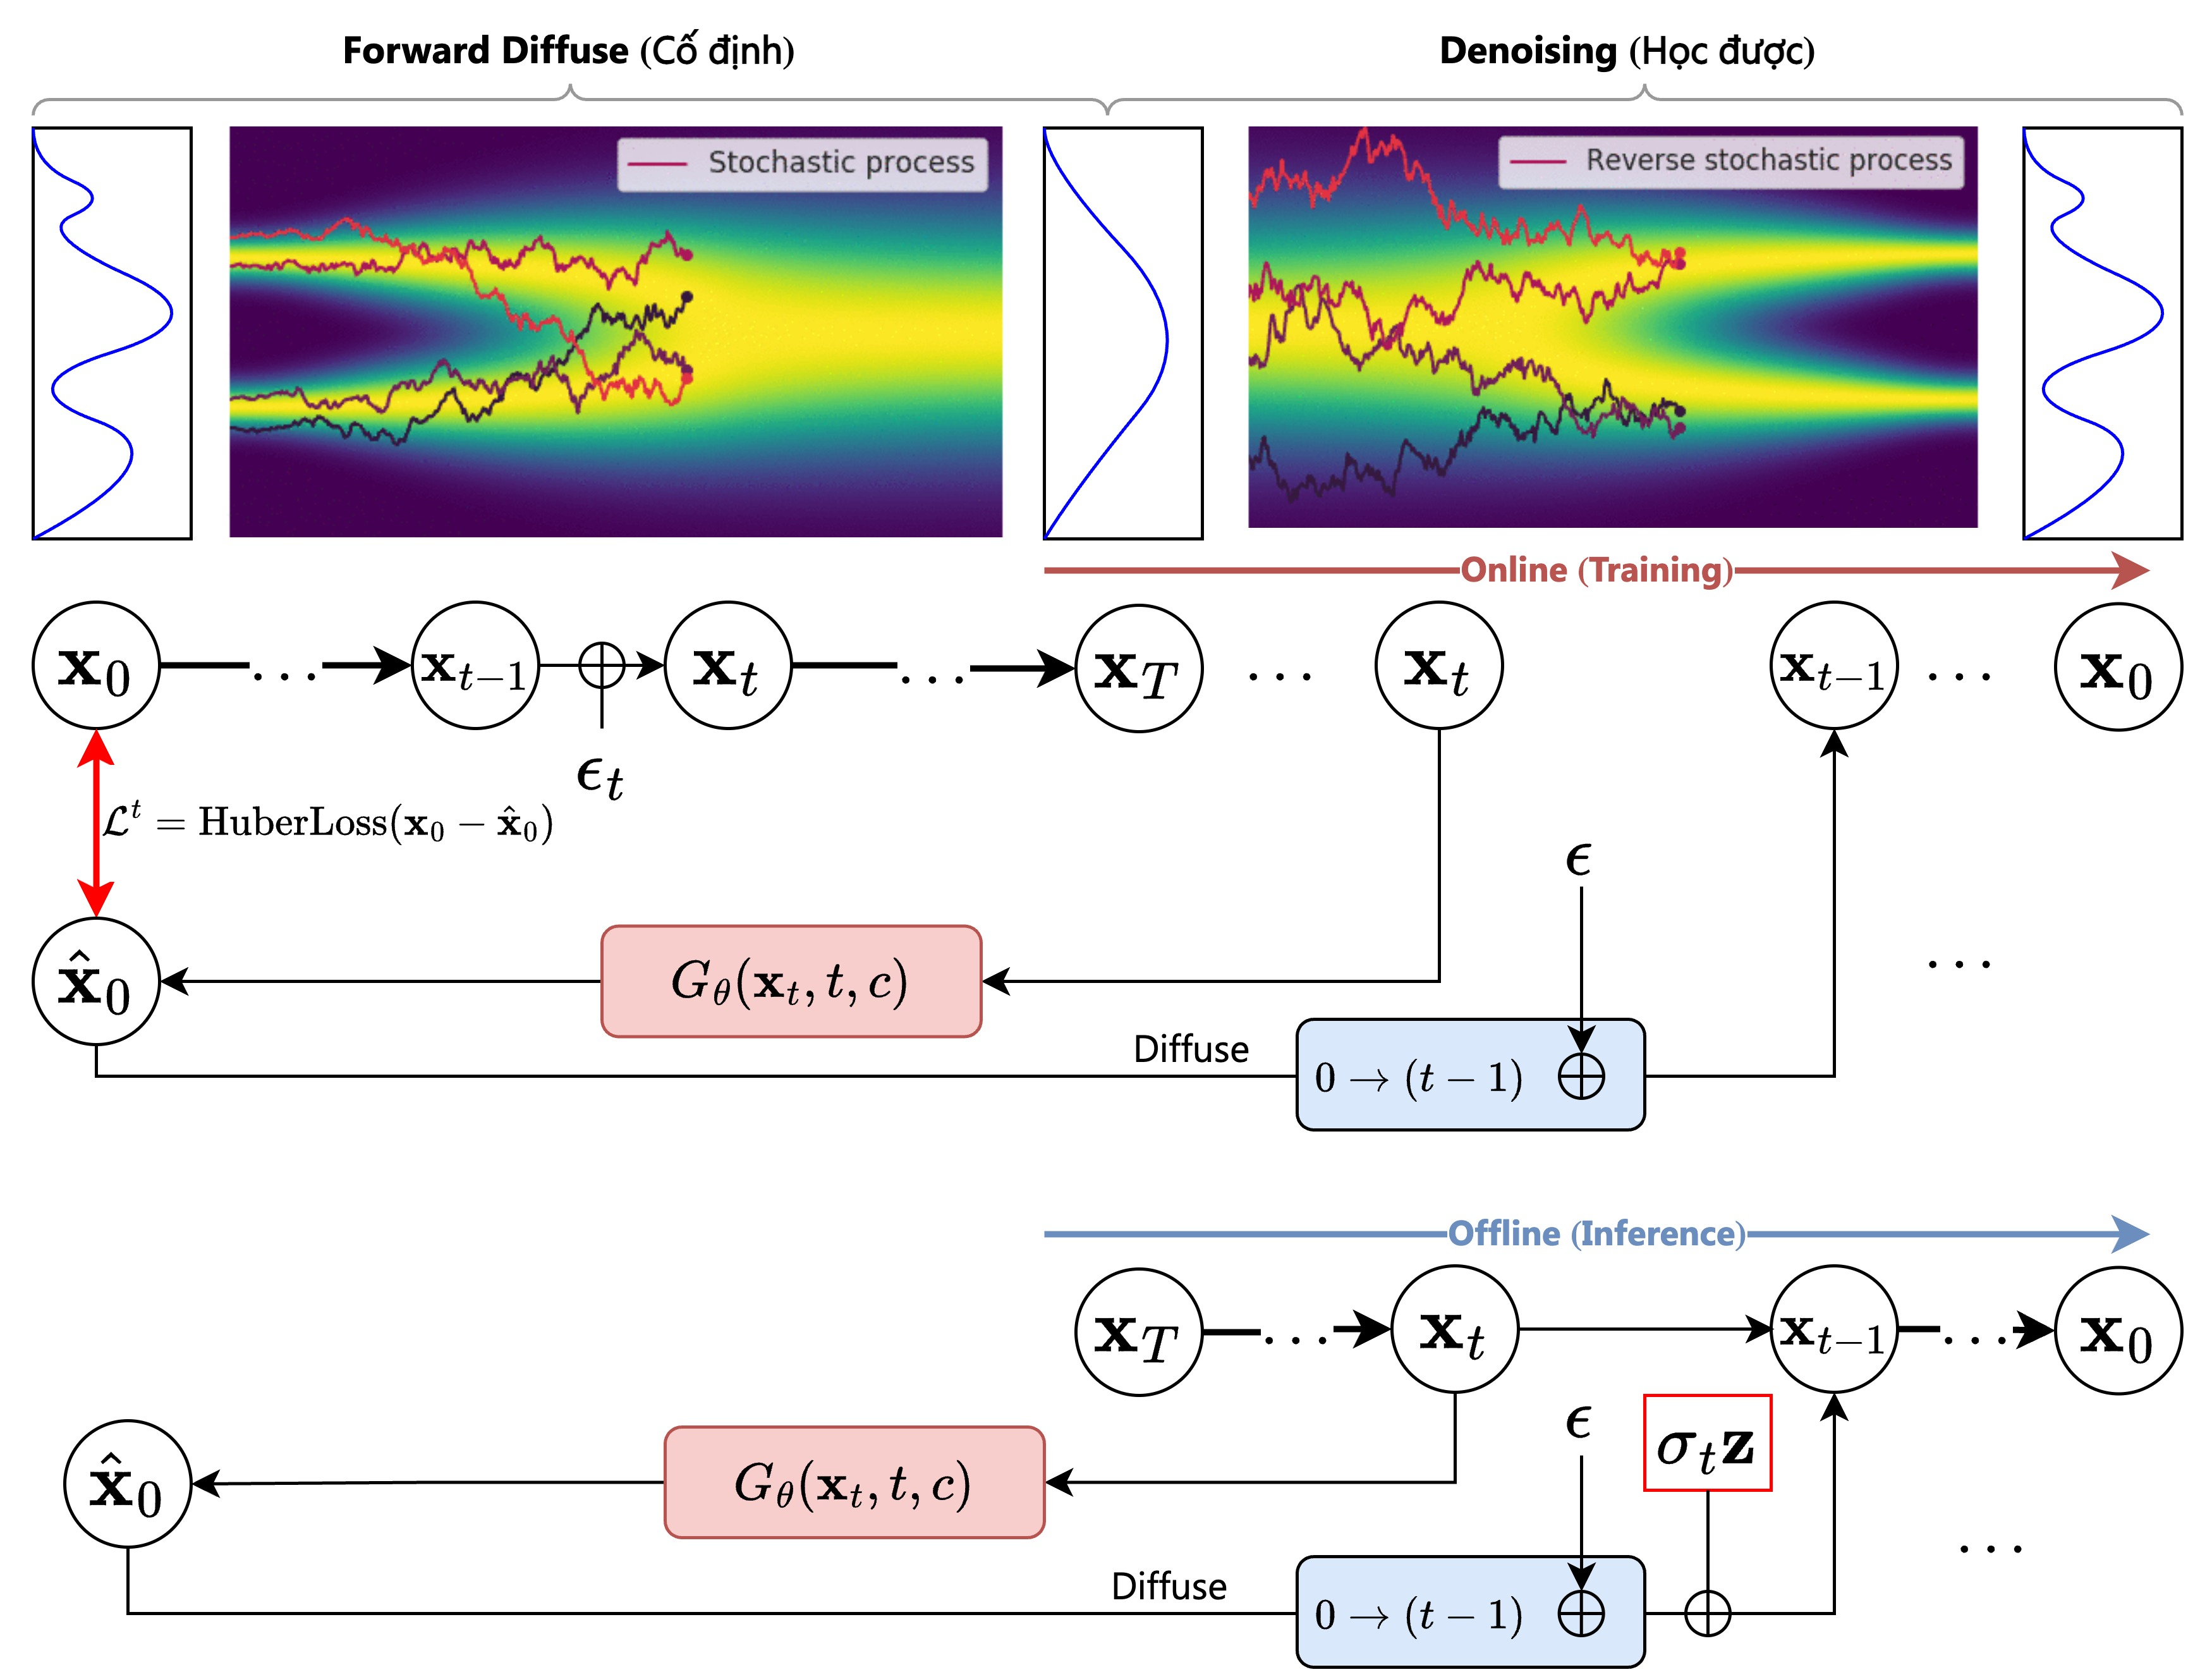
\includegraphics[width=\linewidth]{OnlineAndOffline}
	\caption{Quá trình học Offline (Training) và Online (Inference)}
	\label{fig:OnlineAndOffline}
\end{figure}

Để có thể sinh cử chỉ với chiều dài tùy ý, luận văn cắt chuỗi ban đầu thành các đoạn ngắn có chiều dài $M$. Trong quá trình huấn luyện, cử chỉ khởi tạo đầu tiên có thể được tạo ra bằng cách lấy ngẫu nhiên cử chỉ từ tập dữ liệu hoặc từ lấy trung bình từ đoạn cắt được. Cụ thể ở đây, sẽ lấy góc quay trung bình trong các đoạn đã cắt được. Khi đó, chỉ cần lấy lần lượt các frame đã sinh ra và chọn $N = 8$ frame cuối cùng làm cử chỉ khởi tạo ở lượt tiếp theo. Đối với mỗi đoạn đã cắt ra, cử chỉ $\bx_{t}$ lần lượt sẽ được áp dụng hàm khử nhiều $\hat{\bx}_{0} = G_{\theta'} \left( \bx_{t}, t, c\right)$, sau khi có $\hat{\bx}_{0}$ sẽ được Diffuse (thêm nhiễu) cho đến khi được  $\bx_{t-1}$, và $\bx_{t-1}$ sẽ tiếp tục được làm khử nhiễu cho đến bước khử nhiễu $t=1$ sẽ đạt được $\bx_{0}$ 

\begin{algorithm}
	\caption{Lấy mẫu (sampling) trong OHGesture}
	\label{alg:sampling}
	\setlength{\baselineskip}{10pt}
	\begin{enumerate}
		\item Khởi tạo với nhiễu: $\mathbf{x}_T \sim \mathcal{N}(0, \mathbf{I})$.
		
		\item Các giá trị $\sqrt{\alpha_t}$, $\sqrt{1 - \alpha_t}$ và $\sqrt{\bar{\alpha}_t}$ lấy từ quá trình huấn luyện, tính sẵn giá trị $\sigma_t$ từ $\alpha_t$ ở mỗi bước $t: 1 \rightarrow T$.
		
		\item Chia mỗi đoạn giọng nói 4 giây thành: $\mathbf{a} \in \mathbb{R}^{64000}$. Cử chỉ khởi tạo $\mathbf{s}$ ban đầu là trung bình dữ liệu, sau đó được lấy từ đoạn cử chỉ đã suy luận. Chọn cảm xúc mong muốn, văn bản được lấy từ giọng nói chuyển mã $\mathbf{a}$, tạo cặp điều kiện $c = [\mathbf{s}, \mathbf{e}, \mathbf{a}, \mathbf{v}]$.
		
		\item Với mỗi $t$, lấy $t$ \textbf{tuần tự} từ $[T, \dots, 1]$.
		
		\item Tạo nhiễu ngẫu nhiên $\mathbf{z} \sim \mathcal{N}(0, \mathbf{I})$.
		
		\item Đưa $\mathbf{x}_t$ vào để suy luận $\hat{\mathbf{x}}_0^{(t)} = G_{\theta'}(\mathbf{x}_t, t, c)$.
		
		\item Thực hiện thêm nhiễu $\hat{\mathbf{x}}_0^{(t)}$ từ bước $0 \rightarrow t$ để nhận $\hat{\mathbf{x}}_{t-1}^{(t)}$.
		
		\item Cộng thêm nhiễu: $\hat{\mathbf{x}}_{t-1} = \hat{\mathbf{x}}_{t-1}^{(t)} + \sigma_t \mathbf{z}$.
		
		\item Quay lại bước 4. Khi $t = 1$, thu được $\hat{\mathbf{x}}_0$ từ quá trình khử nhiễu.
	\end{enumerate}

\end{algorithm}

\autoref{alg:sampling} lấy mẫu bắt đầu bằng việc khởi tạo cử chỉ nhiễu ban đầu $\mathbf{x}_T$ từ phân phối chuẩn $\mathcal{N}(0, \mathbf{I})$. Sau đó, các giá trị $\sqrt{\alpha_t}$, $\sqrt{1 - \alpha_t}$ và $\sqrt{\bar{\alpha}_t}$ được lấy từ quá trình huấn luyện, cùng với giá trị $\sigma_t$ được tính từ $\alpha_t$ tại mỗi bước thời gian $t$ từ 1 đến $T$. Mỗi đoạn giọng nói 4 giây được chia thành các chuỗi dữ liệu $\mathbf{a}$, và cử chỉ khởi tạo $\mathbf{s}$ được lấy từ trung bình dữ liệu hoặc từ đoạn cử chỉ đã suy luận. Cảm xúc mong muốn và văn bản được lấy từ giọng nói chuyển mã $\mathbf{a}$, tạo thành một cặp điều kiện $c = [\mathbf{s}, \mathbf{e}, \mathbf{a}, \mathbf{v}]$. Thuật toán sau đó thực hiện các bước tuần tự, bắt đầu từ bước cuối cùng $T$ và tiến ngược về 1. Ở mỗi bước, nhiễu ngẫu nhiên $\mathbf{z}$ được tạo ra và mô hình dự đoán $\hat{\mathbf{x}}_0^{(t)}$ từ cử chỉ nhiễu $\mathbf{x}_t$, thời gian $t$, và cặp điều kiện $c$. Dự đoán này được chuyển tiếp để tính toán $\hat{\mathbf{x}}_{t-1}^{(t)}$ cho bước tiếp theo, và nhiễu được cộng vào để cập nhật cử chỉ tại bước $t-1$. Quá trình này lặp lại cho đến khi đạt đến bước 1, khi đó thuật toán thu được cử chỉ khử nhiễu $\hat{\mathbf{x}}_0$ như là kết quả dự đoán cuối cùng.
